\documentclass[10pt]{article}
\usepackage{icmlko}

\icmlmeta{IP 파운데이션 월드모델}{304}{다섯 건이 답을 정하고 있었다}{피처 층에도 위약을 붙였다 --- 답이 갈리는 것 같았는데 갈라 보니 척도가 답을 정하고 있었다}

\begin{document}

\twocolumn[
\icmlheader

\begin{abstract}
노트 302가 신호 층의 이득이 \emph{내용}이 아니라 \emph{모양}이라는 것을 보고
``절제(지우기)는 내용과 모양을 같이 지운다 --- 시장층 · 피처도 다시 재야
한다''로 끝났다. 피처에 같은 위약을 붙였다(파생피처 다섯을 앵커 사이에서
치환 · 짝 잔존 2/229 · 씨앗 4321). 재기 전에 예측을 ``\textbf{신호와 같을
것 --- 모양}''으로 적었고, 결과를 보기 전에 피처가 앵커 성과를 못 가른다는
것도 확인해 뒀다(IP 회차만 $\rho{=}0.192$ 인데 카테고리 통제 후 0.074).
사전 등록한 척도로 읽으면 \textbf{정반대가 나온다} --- 피처는
\textbf{내용} $t{=}{+}2.21$ · 모양 $t{=}{-}1.21$ 이고 신호는 내용 $-$0.59 ·
\textbf{모양} $+$2.52 다. \textbf{예측이 틀렸다.} 그런데 여기서 멈추면
안 된다(노트 133). 짝 승패를 세니 피처 ``내용''이 \textbf{21 대 21}이고 짝
로그비 중앙이 \textbf{정확히 0.0000} 이다. 절대값 상위 다섯 건이 총합의
43\%를 지고, \textbf{그 다섯을 빼면 $t$ 가 $+$2.21 에서 $+$0.60 으로}
무너진다. 신호 ``모양''도 $+$2.52 $\to$ $+$1.09 다. 다섯 건을 보니
\textbf{전부 진짜 팔의 APE 가 정확히 0.000} --- 사전 등록한 완충 0.05 가
$\log\frac{0.70+0.05}{0+0.05}{=}2.71$ 을 만든다. \textbf{척도가 ``정확히
맞힌 횟수''를 재고 있었다.} 사전 등록의 미리 적은 실패 그대로 ``둘 다 문턱
미달이면 갈랐다고 하지 않는다''를 적용하면 \textbf{피처는 못 가른다}
(2.21 < 2.24). 그리고 신호도 이제는 \textbf{꼬리에 걸려 있다.}
\end{abstract}
]

\section{예측을 적고 쟀고, 틀렸다}

노트 302의 남은 것 첫 줄이 ``시장층 · 피처에 위약''이었다. 피처에 붙였다 ---
\texttt{trust} · \texttt{weekend\_share} · \texttt{holiday\_days} ·
\texttt{ip\_hist} · \texttt{cap\_type} 다섯을 앵커 사이에서 통째로 치환한다
(주변 분포 동일 · 짝 잔존 2/229 · 씨앗 4321 · 시점으로 자른 뒤에 섞음).

\paragraph{미리 적은 것} ``\textbf{신호와 같을 것이다 --- 모양} 쪽에 기운다.''
그리고 결과 보기 전에 근거도 적었다 --- 피처 여섯 중 앵커 일평균과 $p{<}0.05$
인 것은 IP 회차/초회뿐이고($\rho{=}\pm$0.19) \textbf{카테고리를 통제하면
사라진다}(0.074 · $p{=}0.30$).

\begin{center}\footnotesize
\begin{tabular}{lrrl}
\hline
비교 & 효과 & $t$ & \\
\hline
\textbf{피처 · 내용} & $+$0.2349 & \textbf{$+$2.21} & 미달(2.24) \\
피처 · 모양 & $-$0.0907 & $-$1.21 & 미달 \\
\hline
신호 · 내용 & $-$0.0763 & $-$0.59 & 미달 \\
\textbf{신호 · 모양} & $+$0.2843 & \textbf{$+$2.52} & 통과 \\
\hline
\end{tabular}
\end{center}

\textbf{부호가 정반대다.} 피처는 내용 쪽, 신호는 모양 쪽. 예측이 틀렸다.

\section{갈랐더니 척도가 나왔다}

\begin{figure*}[t]
\centering
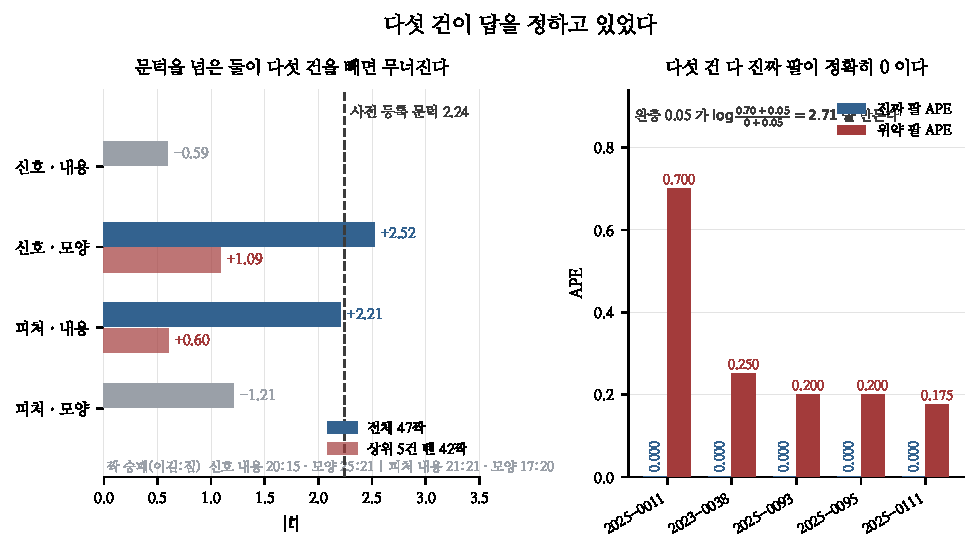
\includegraphics[width=\textwidth]{figs/twice.pdf}
\caption{왼쪽 --- 네 비교의 $|t|$ 와, 절대값 상위 다섯 건을 뺐을 때.
오른쪽 --- 그 다섯 건.}
\end{figure*}

첫 수치를 그대로 채택하지 않는다(노트 133). 같은 짝을 다르게 세 봤다.

\begin{center}\footnotesize
\begin{tabular}{lrrr}
\hline
& 평균 $t$ & 짝 승패 & 짝 로그비 중앙 \\
\hline
피처 · 내용 & $+$2.21 & \textbf{21 : 21} & \textbf{0.0000} \\
신호 · 모양 & $+$2.52 & 25 : 21 & $+$0.0747 \\
신호 · 내용 & $-$0.59 & 20 : 15 & 0.0000 \\
피처 · 모양 & $-$1.21 & 17 : 20 & 0.0000 \\
\hline
\end{tabular}
\end{center}

\textbf{피처 ``내용''은 21 대 21 이고 중앙이 0 이다.} 평균만 크다.

\begin{center}\small
\begin{tabular}{lrr}
\hline
& 전체 47짝 & 상위 5건 뺀 42짝 \\
\hline
피처 · 내용 & $+$2.21 & \textbf{$+$0.60} \\
신호 · 모양 & $+$2.52 & \textbf{$+$1.09} \\
\hline
\end{tabular}
\end{center}

\textbf{둘 다 무너진다.}

\paragraph{그 다섯 건이 무엇인가}

\begin{center}\footnotesize
\begin{tabular}{lrrr}
\hline
레코드 & 진짜 & 위약 & 로그비 \\
\hline
MKT-2025-0011 & \textbf{0.000} & 0.700 & $+$2.708 \\
MKT-2023-0038 & \textbf{0.000} & 0.250 & $+$1.792 \\
MKT-2025-0093 & \textbf{0.000} & 0.200 & $+$1.609 \\
MKT-2025-0095 & \textbf{0.000} & 0.200 & $+$1.609 \\
MKT-2025-0111 & \textbf{0.000} & 0.175 & $+$1.504 \\
\hline
\end{tabular}
\end{center}

\textbf{다섯 건 다 진짜 팔의 APE 가 정확히 0.000 이다.} 사전 등록한 완충
0.05 가 그것을 $\log\frac{0.70+0.05}{0+0.05}{=}2.708$ 로 키운다.

\begin{center}\small
\textbf{척도가 ``정확히 맞힌 횟수''를 재고 있었다.}
\end{center}

\section{그래서 무엇이 남나}

\paragraph{① 사전 등록한 규칙대로 판정한다} 미리 적은 것이 ``둘 다 문턱
미달이면 `갈랐다'고 하지 않는다''였다. \textbf{피처는 못 가른다}(내용 2.21 ·
모양 $-$1.21, 문턱 2.24). 완충을 바꾸면 답이 바뀌겠지만 \textbf{바꾸지
않는다} --- 그것도 미리 적었다.

\paragraph{② 노트 302도 약해진다} 신호 ``모양'' $t{=}2.52$ 는 사전 등록 문턱을
넘었고 그 판정은 유효하다. 다만 \textbf{상위 다섯을 빼면 1.09} 이고
승패가 25:21 이다. \textbf{짝 로그비 중앙이 $+$0.0747 로 0 이 아니라는 점}이
피처와 다른 유일한 자리다 --- 신호 쪽이 조금 더 고르게 퍼져 있다.

\paragraph{③ 척도 선택의 이력} 노트 295가 \emph{더하기} 척도의 꼬리를 보고
(상위 3건이 52$\sim$71\%) \emph{배수} 척도로 옮겼다. 배수가 낫긴 했다 ---
상위 3건이 26$\sim$28\%다. \textbf{그런데 여전히 꼬리가 답을 정한다.}
그리고 배수 척도의 꼬리는 \emph{완충값}이 만든다.

\begin{center}\footnotesize
\begin{tabular}{lll}
\hline
척도 & 상위 3건 몫 & 꼬리를 만드는 것 \\
\hline
더하기 (노트 295) & 52$\sim$71\% & 큰 APE \\
배수 (노트 298$\sim$304) & 26$\sim$28\% & \textbf{APE ${=}$ 0} \\
\hline
\end{tabular}
\end{center}

\paragraph{남은 것}
\begin{center}\small
\begin{tabular}{ll}
\hline
갈래 & 왜 \\
\hline
APE 0 이 왜 생기나 & 47짝에 다섯 건 \\
승패만 보는 척도 & 부호 검정은 꼬리에 안 흔들린다 \\
시장층 위약 & 셋째 층 --- 아직 안 붙였다 \\
표본을 더 & 47짝으로는 꼬리를 못 이긴다 \\
\hline
\end{tabular}
\end{center}

\paragraph{규약} \textbf{척도를 미리 고정해도 그 척도의 꼬리는 안 고정된다.}
노트 298이 척도를 사전 등록해 ``이번에는 척도 고르기가 아니다''라고 적었고
그건 맞다. 그런데 \textbf{고정한 척도가 무엇을 재고 있는지는 여전히 물어야
한다} --- 완충 0.05 는 $\log 0$ 을 막으려고 넣은 값인데, 그 값이 ``정확히
맞힘''을 다른 어떤 개선보다 크게 만든다. \textbf{그리고 평균 옆에 승패와
중앙값을 같이 적어라} --- 21:21 과 $t{=}2.21$ 이 같은 자료다.

\end{document}
